\documentclass[11pt,a4paper]{article}

% ========================================
% PACKAGES
% ========================================
\usepackage[utf8]{inputenc}
\usepackage[T1]{fontenc}
\usepackage{lmodern}  % Better font support for larger sizes
\usepackage[english]{babel}  % Change to your language
\usepackage[margin=2.5cm]{geometry}

% Mathematics
\usepackage{amsmath, amssymb, amsthm}
\usepackage{mathtools}

% Graphics and colors
\usepackage{graphicx}
\usepackage{xcolor}
\usepackage{tikz}
\usetikzlibrary{positioning, arrows.meta, shapes.geometric, calc}
\usepackage{pgfplots}
\pgfplotsset{compat=1.18}
\usepackage[most]{tcolorbox}

% Lists and formatting
\usepackage{enumitem}
\usepackage{parskip}
\usepackage{fancyhdr}

% Code listings (if needed)
\usepackage{listings}

% Hyperlinks
\usepackage{hyperref}
\hypersetup{
    colorlinks=true,
    linkcolor=blue,
    urlcolor=blue,
    citecolor=blue
}

% ========================================
% THEOREM ENVIRONMENTS
% ========================================
\theoremstyle{definition}
\newtheorem{definition}{Definition}[section]
\newtheorem{example}{Example}[section]
\newtheorem{exercise}{Exercise}[section]

\theoremstyle{plain}
\newtheorem{theorem}{Theorem}[section]
\newtheorem{lemma}[theorem]{Lemma}
\newtheorem{proposition}[theorem]{Proposition}
\newtheorem{corollary}[theorem]{Corollary}

\theoremstyle{remark}
\newtheorem*{remark}{Note}
\newtheorem*{observation}{Observation}

% ========================================
% CUSTOM COMMANDS
% ========================================
\newcommand{\R}{\mathbb{R}}
\newcommand{\N}{\mathbb{N}}
\newcommand{\Z}{\mathbb{Z}}
\newcommand{\Q}{\mathbb{Q}}
\newcommand{\C}{\mathbb{C}}

% ========================================
% TABLE OF CONTENTS DEPTH
% ========================================
\setcounter{tocdepth}{2} % Show only parts, sections, and subsections

% ========================================
% HEADER AND FOOTER
% ========================================
\setlength{\headheight}{14pt}
\pagestyle{fancy}
\fancyhf{}
\lhead{\leftmark}
\rhead{AI and Finance}
\cfoot{\thepage}
\renewcommand{\sectionmark}[1]{\markboth{#1}{}}

% ========================================
% DOCUMENT INFORMATION
% ========================================
\title{\textbf{AI and Finance}\\
\large Artificial Intelligence}
\author{Cesare Fraccaroli}
\date{II Semester 2025-2026}

% ========================================
% DOCUMENT
% ========================================
\begin{document}

\maketitle
\tableofcontents
\newpage

\section{AI \& Finance Summary}

In the first part of the course, we will consider the calibration of parameters for 
stochastic models.

\subsection{Data from the market}
The idea: Given some data from the market
\begin{itemize}
    \item past prices of stocks, bonds ...
    A bond is a piece of paper that promises to pay a certain amount of money at a certain date.
    You can buy a bond for a certain price and in the given date you will receive the money
    (considering an interest rate).
    Stocks are instead a share of a company. You have "no idea" of the future value of the company,
    you can only buy and sell them on the market.
    Prices contain information about the market.
    \item past interest rates. It changes over time and depends on market, company policy, etc.
    Interest rates are fundamental because they allow us to compare amounts of money at different points in time.
    \item option prices (call and put options). 
    An option is a contract that gives the right to buy or sell a certain asset at a
    certain price at a certain date.
    Call option: gives the right to buy an asset at a certain price at a certain date.
    Put option: gives the right to sell an asset at a certain price at a certain date.
    It is a sort of insurance.
    This option are very liquid, meaning that they can be bought and sold very easily.
    Example: you want to buy steel in the future, but you think that the price will increase.
    You can buy a call option on steel. If the price of steel increases, 
    you can exercise the option and buy steel at the price of the option.
    If the price of steel decreases, you can let the option expire and lose the money you paid for the option.
    Example: you want to sell steel in the future, but you think that the price will decrease.
    You can buy a put option on steel. If the price of steel decreases, 
    you can exercise the option and sell steel at the price of the option.
    

\end{itemize}
These are all important types of data that we can use to calibrate parameters for stochastic models.

\subsection{Stochastic Models}
In finance there is a part of the description that is \emph{deterministic}, but there is also a part that is \emph{stochastic}.
For example, we can consider the \textbf{Bernoulli model}.
\subsubsection{Bernoulli Model}
\begin{figure}[h!]
    \centering
    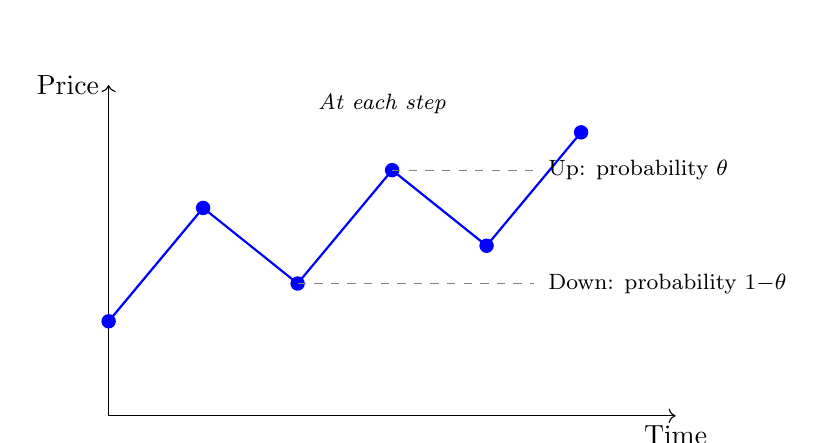
\begin{tikzpicture}[scale=1.2]
        % Axes
        \draw[->] (0,0) -- (6,0) node[below] {Time};
        \draw[->] (0,0) -- (0,3.5) node[left] {Price};
        
        % Bernoulli "spiky" price path
        \draw[thick, blue]
            (0,1) -- (1,2.2) % up
            -- (2,1.4) % down
            -- (3,2.6) % up
            -- (4,1.8) % down
            -- (5,3); % up

        % Points
        \foreach \x/\y in {0/1, 1/2.2, 2/1.4, 3/2.6, 4/1.8, 5/3} {
            \filldraw[blue] (\x,\y) circle (2pt);
        }

        % Horizontal dashed lines to labels for up and down
        % Up label and dashed line
        \draw[dashed, gray] (3,2.6) -- (4.5,2.6);
        \node[align=left, anchor=west] at (4.55,2.6) {\footnotesize Up: probability $\theta$};

        % Down label and dashed line (now at 1.4 to match lower point)
        \draw[dashed, gray] (2,1.4) -- (4.5,1.4);
        \node[align=left, anchor=west] at (4.55,1.4) {\footnotesize Down: probability $1{-}\theta$};

        % Optional: description
        \node at (2.9,3.3) {\footnotesize \textit{At each step}};
    \end{tikzpicture}
    \caption{Bernoulli model: at each step, price can go up (probability $\theta$) or down (probability $1{-}\theta$).}
\end{figure}

\subsubsection{Black-Scholes Model}
The \textbf{Black--Scholes model} is a stochastic model that describes the price of a stock over time.
It is a continuous-time model used to price options.
It is more complex than the Bernoulli model, but also more accurate.
It is based on the assumption that the price of a stock follows a \emph{geometric Brownian motion}.
Ignoring the interest rate for the moment, we can write:

\begin{tcolorbox}[colback=blue!3!white,colframe=blue!60!black,title={\textbf{Black--Scholes dynamics (no drift)}}]
In differential notation, the Black--Scholes model expresses the evolution of the asset price $S$ as
\begin{equation}
    dS_t = S_t \, \sigma_{BS} \, dW_t,
\end{equation}
where:
\begin{itemize}
    \item $S_t$ is the asset price at time $t$,
    \item $\sigma_{BS}$ is the volatility coefficient (a measure of how much the price can fluctuate),
    \item $dW_t$ is an increment of a Wiener process (standard Brownian motion).
\end{itemize}
In a small time step $\delta t$, a discretised version can be written as
\begin{equation}
    S_{t+\delta t} = S_t + S_t \, \sigma_{BS} \, (W_{t+\delta t} - W_t),
\end{equation}
where $W_{t+\delta t} - W_t$ is again an increment of Brownian motion.
\end{tcolorbox}

We basically add a variance proportional to the time step and to today's price.
The parameter $\sigma_{BS}$ is the volatility coefficient.
A bigger $\sigma_{BS}$ means that the price can fluctuate more, while if $\sigma_{BS}=0$ the price is constant.

There are parameter-dependent (i.e.\ depending on $\sigma_{BS}$) prices of call and
put options for each strike $K$ and maturity $T$.
\begin{equation}
    C^K,T (\sigma_BS, S_0) \quad \& \quad P^K,T (\sigma_BS, S_0)
\end{equation}

\subsubsection{Stochastic Volatility Model}
We can improve the Black--Scholes model by introducing a \emph{stochastic volatility}.
We obtain a more complex model:
\begin{align}
    dS_t \hspace{1.5em} &=\ S_t \sqrt{V_t} \, dW_t' \nonumber \\
    dV_t \hspace{1.5em} &=\ \kappa (\theta - V_t) \, dt + \sigma_{SV} \sqrt{V_t} \, dW_t^{(2)} \nonumber \\
    d\langle W', W^{(2)} \rangle_t &=\ \rho \, dt
\end{align}
where:
\begin{itemize}
    \item $W_t'$ and $W_t^2$ are two independent Wiener processes (standard Brownian motion).
    \item $\kappa$ is the rate of mean reversion,
    \item $\theta$ is the long-term average volatility,
    \item $\sigma_SV$ is the volatility of the volatility.
    \item $\rho$ is the correlation between the two Wiener processes.
\end{itemize}

The increments $(W'_{t+\delta t} - W'_t)$ and $(W^2_{t+\delta t} - W^2_t)$ are jointly normally distributed as
\[
\mathcal{N}\left(
    0,
    \delta t \begin{pmatrix}
        1 & \rho \\
        \rho & 1
    \end{pmatrix}
\right).
\]
This leads to complicated parameter-dependent prices for call and put options.
The goal is to find the best possible parameters for the model.
\begin{itemize}
    \item Matching the observations on the market
    \item In a quick way
\end{itemize}

How can we do this?
Typically with \textbf{regressions}, for example:
\begin{itemize}
    \item classical approach: maximum likelihood estimation (MLE),
    \item Gaussian processes,
    \item neural networks.
\end{itemize}

\subsection{Implied volatility and inverse pricing}

What do we need to learn?
We want to learn the mapping from option prices and, more generally, market data to 
the best possible parameters for the model.
We are especially interested in approximating key functionals such as the \emph{implied volatility}.

\begin{tcolorbox}[colback=green!3!white,colframe=green!50!black,title={\textbf{Pricing and implied-volatility maps}}]
In the Black--Scholes model there is a pricing map
\begin{equation}
    (\sigma_{BS}, S_0) \mapsto C^{K,T}(\sigma_{BS}, S_0),
\end{equation}
and one can (in principle) construct a very complicated inverse map
\begin{equation}
    C^{K,T}(\sigma_{BS}, S_0) \mapsto (\sigma_{BS}, S_0).
\end{equation}
The \emph{implied volatility} is the value of $\sigma_{BS}$ such that the model price $C^{K,T}(\sigma_{BS}, S_0)$
matches the observed market price of the option.
\end{tcolorbox}

If we now fix T:

\begin{figure}[h!]
    \centering
    \begin{tikzpicture}[scale=1.3]
        % Axes
        \draw[->] (0,0) -- (7,0) node[right] {$K$};
        % Vertical axis at the origin
        \draw[->] (0,-0.5) -- (0,5) node[above] {Call price $C$};

        % S_0 label on the right of the x-axis
        \draw[dashed,gray] (4.0,0) -- (4.0,4.8);
        \node[below] at (4.0,0) {$S_0$};

        % Decreasing convex schematic call-price curve
        \draw[thick,blue,domain=0.1:7,samples=100,smooth]
            plot(\x, {3*exp(-0.4*(\x-1))});

        % Annotate regions
        \node at (2,2.7) {\footnotesize ITM};
        \node at (6.2,0.5) {\footnotesize OTM};

        % Mark a schematic point at $K = S_0$
        \fill (4.0,0.74) circle (1.1pt);
        \node[right] at (5.05,0.74) {\scriptsize $C(S_0)$};

        % Axis labels and origin
        \node[below left] at (0,0) {$0$};
    \end{tikzpicture}
    \caption{Schematic plot of the price $C$ of a call option as a function of strike $K$, with $S_0$ located on the right half of the $x$-axis. The blue curve illustrates a decreasing, convex call-price profile.}
    \label{fig:call_price_vs_strike}
\end{figure}
Here we can apply the IV map and get the sigma of the Black-Scholes model.
\begin{figure}[h!]
    \centering
    \begin{tikzpicture}[scale=1.3]
        % Axes
        \draw[->] (0,0) -- (7,0) node[right] {$K$};
        % Vertical axis at the origin
        \draw[->] (0,-0.5) -- (0,7) node[above] {$\sigma_{BS}$};

        % S_0 label on the right of the x-axis
        \draw[dashed,gray] (4.0,0) -- (4.0,6.8);
        \node[below] at (4.0,0) {$S_0$};

        % Volatility "smile": convex curve with minimum at $K = S_0$
        \draw[thick,blue,domain=1.5:6.5,samples=100,smooth]
            plot(\x, {0.7*((\x-4.0)^2)+1.2});

        % Middle horizontal line (green)
        \draw[thick,green!70!black] (0.5,2) -- (6.8,2);

        % Label for green line (constant Black--Scholes volatility)
        \node[right, green!70!black] at (6.85,2) {\footnotesize Constant $\sigma_{BS}$};

        % Highlight S_0 intersection (minimum of the smile)
        \filldraw[blue] (4.0,1.2) circle (1.2pt);
        \node[below left] at (4.0,1.2) {\scriptsize $(S_0, \min \sigma_{BS})$};

        % Axis labels and origin
        \node[below left] at (0,0) {$0$};
    \end{tikzpicture}
    \caption{Schematic plot of implied volatility $\sigma_{BS}$ as a function of strike $K$, with $S_0$ placed on the right half of the $x$-axis. The blue curve illustrates the volatility "smile" often observed in implied volatility, while the horizontal green line marks the constant Black--Scholes volatility.}
    \label{fig:iv_smile}
\end{figure}
This is usually called the \emph{volatility smile}.
Often one prefers to replace prices with the implied volatility, since volatility is naturally scaled and still interpretable. 
More generally, we can view option prices as \emph{pricing functionals} for complicated stochastic models or exotic options,
mapping model parameters to theoretical prices.

Universal approximation theorem(s)

\section{Time Series (second part of the course)}

Given observations of available quantities over time:
\begin{itemize}
    \item prices of stocks, 
    \item bonds, 
    \item options, 
    \item interest rates
    \item historical values of variance and covariance
    \item historical values of traded volumes
\end{itemize}

Goal: \textbf{forecast} the next value of the corresponding quantity together with the corresponding \emph{uncertainty}.

How: studying the time series (frequency, autocorrelation, stationarity, \dots)
\begin{enumerate}
    \item Apply an econometric model:
    \begin{itemize}
        \item ARMA($p$, $q$) model:
        \begin{itemize}
            \item $Y_t = \mu + \sum_{i=1}^p \phi_i Y_{t-i} + \sum_{j=1}^q \theta_j \epsilon_{t-j} + \epsilon_t$
            \item where:
            \begin{itemize}
                \item $Y_t$: observation at time $t$ (arrow above $Y_{t-i}$: "past observation")
                \item $\epsilon_t$: random shock/innovation at time $t$ (arrow above both $\epsilon$'s: "shocks")
            \end{itemize}
        \end{itemize}
        \item GARCH model:
        \begin{itemize}
            \item calibration
            \item evaluation of performance
        \end{itemize}
    \end{itemize}
    \item Apply a RNN (recurrent neural network):
    \begin{itemize}
        \item calibration (training)
        \item evaluation of performance (testing)
    \end{itemize}
\end{enumerate}
\subsection{Main applications}
\begin{itemize}
    \item Risk estimation of given portfolios 
    (how can one measure risk?)
    \begin{itemize}
        \item variance;
        \item \textbf{Value at Risk (VaR)}: e.g.\ $\text{VaR}_{99\%} = 100$ if and only if the probability of having a loss $\ge 100$ is approximately $1\%$;
        \item \textbf{Expected Shortfall (ES)}: expected loss \emph{conditional} on VaR being exceeded. This is typically called \textbf{CVaR} in engineering.

    \end{itemize}
\end{itemize}
We use these models to forecast the distribution (mean, variance, \dots) of the value of a portfolio
and use it to compute the corresponding risk. 
We then backtest the obtained predictions and perform portfolio optimization (e.g.\ \emph{Markowitz} and \emph{Reinforcement Learning} approaches).
\end{document}